% Grafo ponderado com um caminho destacado
% Feito para o ÉguaTeX (eguatex.com.br). Uso livre (CC0 1.0).
%
% Compile e pronto: sai só a figura, em PDF.
% Para pôr no seu trabalho, use o PDF com \includegraphics ou copie
% o bloco tikzpicture para dentro de uma figure.
%
% No exemplo, o caminho destacado é o mais curto de A até F (custo 11).
\documentclass[tikz,border=4pt]{standalone}
\usepackage[T1]{fontenc}
\usepackage{lmodern}

\colorlet{corCaminho}{red!75!black}

\begin{document}
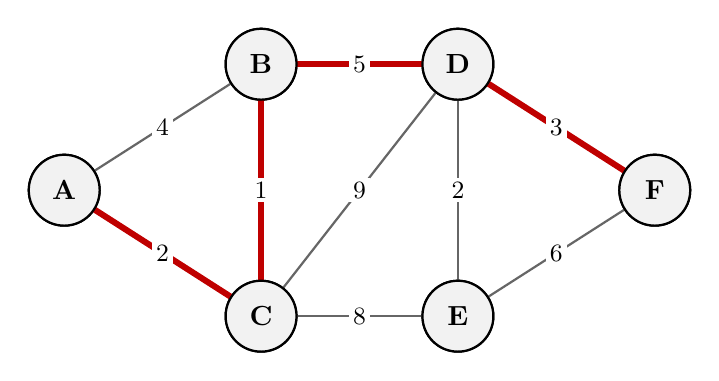
\begin{tikzpicture}[line cap=round, line join=round,
  vertice/.style={circle, draw, line width=0.8pt, fill=black!5, minimum size=0.9cm, font=\bfseries},
  aresta/.style={line width=0.8pt, black!60},
  destaque/.style={line width=2.2pt, corCaminho},
  peso/.style={fill=white, inner sep=1.5pt, font=\small}]

% Vértices: nome/posição (x, y em cm).
\def\vertices{A/{(0,0)}, B/{(2.5,1.6)}, C/{(2.5,-1.6)}, D/{(5,1.6)}, E/{(5,-1.6)}, F/{(7.5,0)}}
% Arestas: de/para/peso.
\def\arestas{A/B/4, A/C/2, B/C/1, B/D/5, C/E/8, C/D/9, D/E/2, D/F/3, E/F/6}
% Caminho destacado: arestas em sequência, de/para.
\def\caminho{A/C, C/B, B/D, D/F}

\foreach \n/\pos in \vertices \node[vertice] (\n) at \pos {\n};
\foreach \u/\v/\w in \arestas \draw[aresta] (\u) -- (\v) node[peso, midway] {\w};
\begin{scope}[on background layer/.try]
  \foreach \u/\v in \caminho \draw[destaque] (\u) -- (\v);
\end{scope}
\foreach \n/\pos in \vertices \node[vertice] at \pos {\n};
\foreach \u/\v/\w in \arestas \path (\u) -- (\v) node[peso, midway] {\w};
\end{tikzpicture}
\end{document}
